\begin{trapbox}
\textbf{易错1：不判断点与圆的位置。}
统一结论（圆周距离）：$\min PA=|d-R|$，$\max PA=d+R$。
\begin{itemize}
\item 圆外 $d>R$：最小值 $d-R$。
\item 圆上 $d=R$：最小值 $0$。
\item 圆内 $0<d<R$：最小值 $R-d$。
\item 圆心 $d=0$：所有圆周点距离均为 $R$，不再有唯一极值点。
\end{itemize}\begin{center}
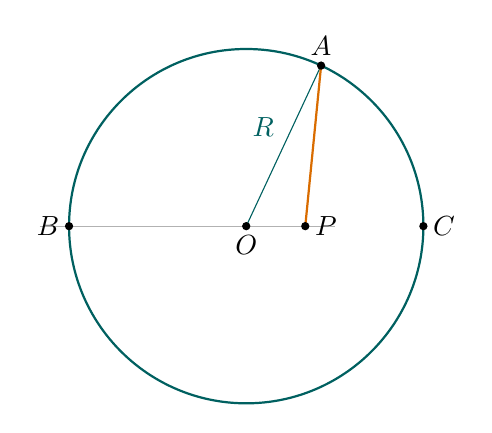
\begin{tikzpicture}[scale=.75,>=stealth]
 \coordinate (O) at (0,0); \coordinate (P) at (1,0);
 \coordinate (A) at (65:3); \coordinate (C) at (3,0); \coordinate (B) at (-3,0);
 \draw[gray!60] (-3.5,0)--(1.5,0);
 \draw[teal!75!black,thick] (O) circle (3);
 \draw[teal!75!black] (O)--(A) node[midway,above left] {$R$};
 \draw[orange!85!black,thick] (P)--(A);
 \fill (O) circle (2pt) node[below] {$O$};
 \fill (P) circle (2pt) node[right] {$P$};
 \fill (A) circle (2pt) node[above] {$A$}; \fill (C) circle (2pt) node[right] {$C$}; \fill (B) circle (2pt) node[left] {$B$};
 \end{tikzpicture}

\end{center}
\textbf{易错2：混淆圆周与圆盘。} 若动点可在闭圆盘内，则最小距离为 $\max(0,d-R)$；最大距离仍为 $d+R$。

\textbf{易错3：只证明不等式，不验证取等。} 上下界未必是最值，必须说明圆周上确实存在对应点；若动点仅在一段圆弧上，还要检查极值点是否在允许范围内。

\textbf{易错4：认为垂线最短。} 垂线最短适用于点到直线，不能直接替代点到圆周的证明。

\textbf{易错5：开平方漏绝对值。} $\sqrt{(d-R)^2}=|d-R|$，只有在 $d\geqslant R$ 时才能写为 $d-R$。
\end{trapbox}
